\newpage
\section{It's What the Book Says} 
\fixnote{Somehow give a sense that this activity is about definitions.  Include trapezoids, and allow for both definitions. Also rectangles, kites.}

Fifth graders were given the following task: Put the
terms \textbf{square}, \textbf{rhombus}, \textbf{parallelogram}, in
the Venn diagram below.
\[
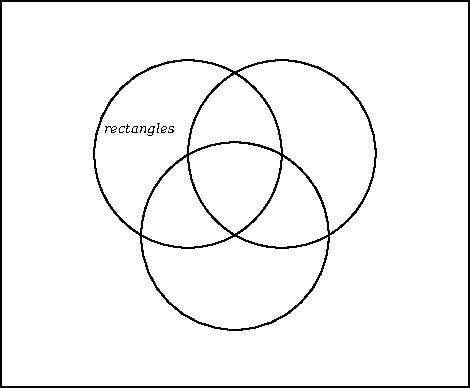
\includegraphics{../graphics/venn.pdf}
\]


\begin{prob} 
What are \textit{squares}, \textit{rhombuses},
and \textit{parallelograms}?
\end{prob}


\begin{prob} 
Critique the question above based on mathematical content.
\end{prob}

\begin{prob} 
Create a Venn diagram showing the correct relationship
between \textit{rectangles}, \textit{squares}, \textit{rhombuses},
and \textit{parallelograms}. Be ready to present and defend your
diagram to your peers.
\end{prob}
